\documentclass[preprint,10pt]{elsarticle} 
%% The graphicx package provides the includegraphics command.
\usepackage{graphicx}
%% The amssymb package provides various useful mathematical symbols
\usepackage{amssymb}
%% The amsthm package provides extended theorem environments
%% \usepackage{amsthm}

%% The lineno packages adds line numbers. Start line numbering with
%% \begin{linenumbers}, end it with \end{linenumbers}. Or switch it on
%% for the whole article with \linenumbers after \end{frontmatter}.
\usepackage{lineno}
\journal{Universidade Federal do Para}

\begin{document}
\begin{frontmatter}

%% Title, authors and addresses
\title{Tools for NDN architectures: ndnSIM vs. NFD}
\author{Igor}
\date{February 2017}
\address{Belem, Brazil}
\begin{abstract}
%% Text of abstract
With the huge increase in data traffic in the nowadays network, the need for the research and development for protocols that suits better this huge traffic is rising and some of the most promising research are in ICN(Information-Centric Networks) areas such as NDN(Named Data Network) protocol, since the main proposal of these protocols is placing the data as the center of the network not the end nodes connection anymore, this way relieving the actual weight that the servers/end-nodes in the IP architecture have to carry to supply the demand of a huge number of accesses. Knowing that the NDN network still has some lacks and issues not solved (such as setting the most feasible implementation of IOT network and ensuring the quality of service in video streamings) due to its state of development, the research needs more productivity to be in an implementable state for being a feasible 5g solution. In order to help the research and development of these protocols, tools for the researchers are needed, tools for simulation and emulation that help the programmers to develop the "ideal algorithms" for these protocols.

\end{abstract}

\begin{keyword}
NFD \sep ndnSIM \sep ICN \sep NDN 
%% keywords here, in the form: keyword \sep keyword

%% MSC codes here, in the form: \MSC code \sep code
%% or \MSC[2008] code \sep code (2000 is the default)

\end{keyword}
\end{frontmatter}
\section{Introduction}
\label{S:1}
   NDN is a very promising architecture that is being developed in the last few years, it aspires to be the successor of the actual most used architecture, the IP architecture, despites being a good solution for many problems that the IP architecture has facing, NDN is still being developed, for that, the academia and the developers need tools to test, study and improve the NDN algorithms, tools preferably, powerful, open source and less complex as possible for the users so the tools can be common, get the wide research community using it and helps the community to develop faster the ideals algorithms for this new architecture. \par
    ndnSIM and NFD are so far the most relevant and used tools in the research and development of NDN networks, each one has its own applications, even usually used together for a more realistic simulation, they are in fact separate things, having each one a different function.
\section{Main Conceipts}
\label{S:2}
\subsection{ndnSIM}
ndnSIM is a network simulator based on the NS-3 simulator~\cite{ndnSIM}, one of the most powerful tools in simulating networks. ndnSIM can be described as a framework built over NS-3 to simulate NDN network, ndnSIM have its applications written in c++ and even though its an application built to simulate NDN networks it uses NFD in its core to implement NDN functions such as PIT's, FIB's and Content Store functions on the nodes. \par
To be more specific, ndnSIM is a simulator that allows a easy configuration of simulated networks through its helpers and allows also a wide range of possible networks topologies since inherits this functions from NS-3, a major tool in networks simulations, but also extends NS-3 having its own libraries to work with NDN networks and implementing NFD/ndn-cxx libraries to work on the core of the nodes making the simulation more near to the realistic results and helping the users since the NDN functions are already written in NFD/ndn-cxx libraries which are deloped by the community effort, this way the user get rid of doing the code for this basic functions.\par  
For that ndnSIM can be described as a indispensable tool for the research of NDN protocol since through that tool it is possible to configure, simulate and track/observe/debug a Named Data Network easily using the helpers, structures inherited from the NS-3 and use a trustable forwarder built and developed also by the community(NFD).\par
Pros:
\begin{itemize}
		\item Built over NS-3 a tool with a large community.
		
		\item Capable of simulating different kinds of networks with different speed, different topologies, different transport methods.
		
		\item Easy configuration of the network that will be simulated.
		
		\item Supports NFD to run in the core of the nodes.
	\end{itemize}
\subsection{NFD}
NFD(NDN Forwarding Daemon) is the NDN "official" network forwarder which implements the forwarding algorithms of this protocol and evolves together with it. It had its first release main developed by the NSF-sponsored NDN project team, but now the project already have significant contributions from the community.\par
NFD can be seen as an official NDN library written to run Named Data Network main functions, NFD is what we can say "the program which will run in the core of the nodes".\par
The most significant modules that NFD implements are:

	\begin{itemize}


         \item The Core Module: module which implements many main services such as DNS resolver, hash computation routines, face monitoring and other services that are shared between different NFD modules
        
        \item The Face Module: responsible for implementing the face abstraction on lower level transport mechanisms. 
        
        \item The Tables: Implements the tables of NDN protocol, Pending Interest Table(PIT), Contest Store(CS), Forwarding Information Base(FIB) and some others structures that help in the Named Data Network forwarding
        
        \item RIB Management: Manages the Routing Information Base(RIB), the RIB is responsible for generating a consistent fowarding table(FIB), for that is a separate module

        \item Forwarding Module: Implements basic packet processing pathways, it interacts with Faces, Tables, and Strategies.
	\end{itemize}

For being a forwarder, not a simulator, NFD can actually be used for emulation, since it is written to run on the core of the nodes, for this reason, NFD does not need ndnSIM to run, NFD can be used separately in the computers or virtual machines in order to emulate NDN networks.\par
This capacity of emulation is a critical point for the researchers since it allows a real implementation of the codes created and developed in simulations, it allows the user, in fact, observe your code running and the differents real nodes actually communicating with each other through the code written for NDN protocol.\par
Pros:
\begin{itemize}
		\item Widely developed by the community.
		
		\item Capable of emulation and can be used by other programs for simulation.
		
		\item Evolve together with the NDN protocol
		
	\end{itemize}
\section{Conclusions}
\label{S:3}
As seen, NFD and ndnSIM are powerful tools built to help the research in Named Data Network area, having each one its main function. While ndnSIM, is a powerful tool to simulate the structure of a wide network, with different topologies and variables in a simple way, NFD allows the nodes to work as actuals NDN nodes with codes developed partially by the community itself.\par
\begin{figure}[ht]
			\centering
			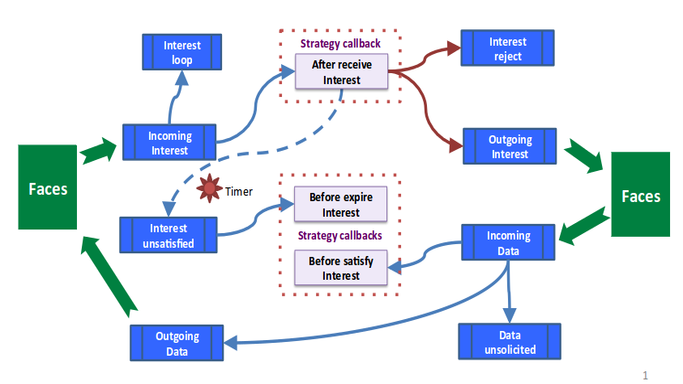
\includegraphics[height=3in, width=3.2in]{./Figures/Pipeline}
			\caption{pipeline illustration of both programs working together in a simulation}
			\label{fig:not_congested_results1}
		\end{figure} 
\end{document}
  